% Selección de la clase del documento - formato IEEE para conferencias
\documentclass[conference]{IEEEtran}

%conjunto de paquetes------------------------------------
% Paquete para soporte de idioma español (hyphenation, traducciones)
\usepackage[spanish]{babel}
% Codificación de caracteres (acentos, ñ, etc.)
\usepackage[utf8]{inputenc}
% Codificación de fuentes para mejor manejo de caracteres especiales
\usepackage[T1]{fontenc}
% Paquete para incluir imágenes (PNG, JPG, PDF)
\usepackage{graphicx}
% Paquete para manejo de referencias bibliográficas
\usepackage{cite}
\usepackage{url} % o mejor aún:
\usepackage{hyperref}
\usepackage{amsmath} % Para entornos matemáticos
\usepackage{amssymb} % Para \mathbb{R}
\usepackage{parskip} % Mejor manejo de espacios entre párrafos
\usepackage{booktabs} % Para \toprule, \midrule, etc.
\usepackage{unicode-math}     % Soporte para símbolos Unicode en matemáticas
\usepackage[breaklinks]{hyperref} % Permite saltos en cualquier punto


% Configuración inicial del documento---------------------
\title{Métodos Númericos Gradiente Descendiente y Newton-Raphson}

\author{
\IEEEauthorblockN{A. Rigoberto}
\IEEEauthorblockA{\textit{Universidad Centroamericana Jose simeon cañas}\\
\texttt{00042220@uca.edu.sv}
}
\and
\IEEEauthorblockN{E. Alexander}
\IEEEauthorblockA{\textit{Universidad Centroamericana Jose simeon cañas}\\
\texttt{00066819@uca.edu.sv}
}
\and
\IEEEauthorblockN{\hspace{2cm}O. Heriberto}
\IEEEauthorblockA{\hspace{2cm}\textit{Universidad Centroamericana Jose simeon cañas}\\
\texttt{\hspace{2cm}00177919@uca.edu.sv}
}
\and
\IEEEauthorblockN{\hspace{1.5cm}Z. Daniela}
\IEEEauthorblockA{\hspace{1.5cm}\textit{Universidad Centroamericana Jose simeon cañas}\\
\texttt{\hspace{1.5cm}00062019@uca.edu.sv}
}
\and
\IEEEauthorblockN{\hspace{1.8cm}Q. Javier}
\IEEEauthorblockA{\hspace{1.8cm}\textit{Universidad Centroamericana Jose simeon cañas}\\
\texttt{\hspace{1.8cm}00062019@uca.edu.sv}
}
}

\begin{document}

% Portada-----------------------
\maketitle

% Resumen----------------------
\begin{abstract}
Este artículo investiga los métodos de optimización en aprendizaje automático, con enfoque en el Gradiente Descendente y Newton-Raphson. Analizamos teóricamente las condiciones de convergencia, estabilidad y tasas de error para ambos algoritmos, demostrando que el Gradiente Descendente alcanza una convergencia lineal $\mathcal{O}(1/\epsilon)$ para funciones convexas con gradiente Lipschitz continuo, mientras que para funciones fuertemente convexas la convergencia mejora a $\mathcal{O}(c^k)$. Presentamos las condiciones de estabilidad ($\eta < 2/L$) y caracterizamos los regímenes inestables mediante análisis del índice de progreso relativo. Comparativamente, el método de Newton-Raphson muestra ventajas en velocidad de convergencia pero requiere condiciones de diferenciabilidad más estrictas. Los resultados teóricos se complementan con análisis de sensibilidad a hiperparámetros, escalabilidad y aplicaciones prácticas en problemas de alta dimensionalidad. Concluimos con recomendaciones para la selección de algoritmos según las propiedades de la función objetivo y requerimientos computacionales.
\end{abstract}

\begin{IEEEkeywords}
optimización convexa, gradiente descendente, Newton-Raphson, tasa de convergencia, aprendizaje automático, condiciones Lipschitz
\end{IEEEkeywords}

% Introducción----------------------------
\section{Introducción a Machine learning}
\IEEEPARstart{E}{n} El machine learning es la ciencia de desarrollo de algoritmos y modelos estadísticos que utilizan los sistemas de computación con el fin de llevar a cabo tareas sin instrucciones explícitas, en vez de basarse en patrones e inferencias. Los sistemas de computación utilizan algoritmos de machine learning para procesar grandes cantidades de datos históricos e identificar patrones de datos. Esto les permite generar resultados con mayor precisión a partir de un conjunto de datos de entrada. Por ejemplo, los científicos de datos pueden entrenar una aplicación médica para diagnosticar el cáncer con imágenes de rayos X a partir del almacenamiento de millones de imágenes escaneadas y diagnósticos correspondientes.

\subsection{¿Como funciona?}
\IEEEPARstart{E}{n} La idea central del machine learning es la existencia de una relación matemática entre cualquier combinación de datos de entrada y salida. El modelo de machine learning no conoce de antemano esta relación, pero puede adivinarla si se le dan suficientes conjuntos de datos. Esto significa que cada algoritmo de machine learning se crea en torno a una función matemática modificable. El principio subyacente puede entenderse así:
\begin{enumerate}
  \item Entrenamos el algoritmo al darle las siguientes combinaciones de entrada y salida (e,s): (2,10), (5,19) y (9,31)
  \item El algoritmo calcula que la relación entre la entrada y la salida es: o=3*i+4
  \item A continuación, le damos la entrada 7 y le pedimos que prediga la salida. Puede determinar automáticamente la salida como 25.
\end{enumerate}

\IEEEPARstart{E}{n} Si bien se trata de conocimientos básicos, el machine learning se centra en el principio de que los sistemas de computación pueden relacionar matemáticamente todos los puntos de datos complejos, siempre y cuando tengan suficientes datos y potencia de computación para procesarlos. Por lo tanto, la precisión de la salida está relacionada directamente con la magnitud de la entrada dada.

% Segunda seccion---------------------------------
\section{Gradiente Descendente}
\subsection{Descripcion y/o deduccion del metodo}

\IEEEPARstart{E}{n} El Gradiente Descendente es un algoritmo de optimización fundamental en el aprendizaje automático, utilizado para minimizar la función de pérdida o error de un modelo. Funciona calculando el gradiente (la derivada) de la función de pérdida con respecto a los parámetros del modelo, como los pesos en una red neuronal. Este gradiente indica la dirección en la que la función de pérdida aumenta más rápidamente. \\\\
En el Gradiente Descendente, se ajustan los parámetros del modelo en la dirección opuesta al gradiente, es decir, “descendiendo” hacia el valor mínimo de la función de pérdida. La magnitud del ajuste se controla por la tasa de aprendizaje. Este proceso se repite iterativamente, actualizando los parámetros paso a paso, hasta que se alcanza un mínimo local o global en la función de pérdida, lo que idealmente corresponde a un modelo bien entrenado y optimizado.

\IEEEPARstart{E}{n}En otras palabras La idea de este tipo de métodos es generar una secuencia de valores \({xk}\), de modo que, la función objetivo disminuya en cada avance de una iteración \(f(xk+1) < f(xk)\), Permite espacios más flexibles hasta alcanzar eventualmente un mínimo. Las propiedades de convexidad de la función objetivo \( f\), y el dominio del problema \( \mathbb{R}^n\), aseguran las condiciones necesarias para la convergencia de la sucesión de valores \( \{x_k\} \) generados por el algoritmo de gradiente descendente. 

En general, los algoritmos de descenso escogen una dirección \(dk \colon Rn\) que satisface la regla \(h \nabla f(x), dki < 0\). Esta regla se puede interpretar geométricamente, como la condición donde el vector \(dk\) forma un ángulo de menos de 90 grados con la dirección de máximo descenso. En el caso del método de gradiente, la dirección corresponde al vector de gradiente negativo 

% salto de linea no olvidar usarlo------------------------------

\(dk = - \nabla f(xk)\). Por consiguiente, el vector de gradiente proporciona la dirección de máximo descenso o mayor tasa de descenso en la zona de evaluación local. No obstante, dependiendo del tipo de problema y función, existen otras opciones para el vector de dirección, por ejemplo, subgradientes (cuando la función es no diferenciable) o métodos que utilizan información de segundo orden como el método de Newton que hace uso del Hessiano \((\nabla2f(xk)) - 1\) y en cada iteración minimiza una aproximación cuadrática de la función

El método de gradiente de máximo descenso genera una secuencia de puntos 
\({xk} \colon Rn\) mediante la siguiente expresión de recurrencia \\\\
\(xk+1 = xk - tk\nabla f(xk), k = 0, 1, 2, ... \)

%----------------------------------------------------------
\subsection{Demostracion de orden convergencia}
La tasa de convergencia proporciona los márgenes teóricos de complejidad donde los algoritmos se desempeñan. Estos bordes se modifican de acuerdo a la estructura del problema donde son aplicados. El peor desempeño (límite superior) queda delimitado por la condición Lipschitz del gradiente, mientras que el mejor desempeño se obtiene, suponiendo, el algoritmo evalúa una función fuertemente convexa con parámetro \(µ > 0\). Ambos limites, pueden ser
determinados mediante una aproximación cuadrática de la función objetivo f, empleando las constantes L y µ como parámetros del factor cuadrático (como se observa en las desigualdades (2.9), (2.10) de abajo). El desempeño de la tasa de convergencia para una función convexa, entonces, se caracteriza por situarse entre ambas condiciones de aproximación cuadrática,
 
\(f(y) \leq f(x) + \nabla f(x)^T(y - x) + \frac{L}{2}\lvert y+x \rvert^\frac{2}{2} \) (2.9)\\\\
\(f(y) \geq f(x) + \nabla f(x)^T(y - x) + \frac{L}{2}\lvert y+x \rvert^\frac{2}{2} \) (2.10)\\\\
De manera equivalente usando el Hessiano para todo x en \( \mathbb{R}^n\)
\[
\mu I \preccurlyeq \nabla^2 f(x) \preccurlyeq L I \tag{(2.11)}
\]

En este sentido, para una función f convexa, suave con gradiente Lipschitz continuo de constante L, se demuestra que la tasa de convergencia del método de gradiente de máximo descenso es lineal o logarítmica.
La demostración se inicia con la desigualdad (2.7), que asegura decrecimiento de la función en cada iteración

\[
f(y) \leq f(x) - \left(1 - \frac{1}{2} t L\right) t \| \nabla f(x) \|^2
\]
\[
= f(x) - \frac{(2 - t L)t}{2} \| \nabla f(x) \|^2
\]

Usando \(\alpha\) como variable auxiliar para el término \((2 - t L)t\) y reemplazando se obtiene:

\[
f(y) \leq f(x) - \frac{\alpha}{2} \| \nabla f(x) \|^2 \tag{(2.12)}
\]

Interesa incluir \(f(x_*)\) en esta desigualdad. Para esto, se puede acotar el valor de \(f(x)\) en torno al valor óptimo de la función \(f(x_*)\). Usando la propiedad de convexidad de la función, se tiene la siguiente aproximación lineal en torno al valor óptimo:

\[
f(x_*) \geq f(x) + \nabla f(x)^T (x_* - x)
\]
\[
f(x) \leq f(x_*) + \nabla f(x)^T (x - x_*)
\]

Reemplazando en la desigualdad anterior (2.12):

\[
f(y) \leq f(x_*) + \nabla f(x)^T (x - x_*) - \frac{\alpha}{2} \| \nabla f(x) \|^2
\]
\[
f(y) - f(x_*) \leq \frac{1}{2\alpha} \left( 2\alpha \nabla f(x)^T (x - x_*) - \alpha^2 \| \nabla f(x) \|^2 \right)
\]
\[
= \frac{1}{2\alpha} \left( 2\alpha \nabla f(x)^T (x - x_*) - \alpha^2 \| \nabla f(x) \|^2 + \| x - x_* \|^2 - \| x - x_* \|^2 \right)
\]
\[
= \frac{1}{2\alpha} \left( \| x - x_* \|^2 - \| x - \alpha \nabla f(x) - x_* \|^2 \right)
\]

Se puede observar que \( y = x - \alpha \nabla f(x) \) es la definición de un paso de gradiente:

\[
f(y) - f(x_{*}) \leq \frac{1}{2\alpha} \left( \|x - x_{*}\|^{2} - \|y - x_{*}\|^{2} \right)
\]

Esta última desigualdad ocurre para cada paso de iteración. Sumando todos los pasos:

\begin{align*}
\sum_{i=1}^{k} (f(x_{i}) - f(x_{*})) &\leq \sum_{i=1}^{k} \frac{1}{2\alpha} \left( \|x_{i-1} - x_{*}\|^{2} - \|x_{i} - x_{*}\|^{2} \right) \\
&\leq \frac{1}{2\alpha} \left( \|x_{0} - x_{*}\|^{2} - \|x_{k} - x_{*}\|^{2} \right)
\end{align*}

La sumatoria del lado derecho se cancela haciendo uso de la suma telescópica. Eliminando el término positivo \( \|x_{k} - x_{*}\|^{2} \) permite dejar la diferencia \( \|x_{0} - x_{*}\|^{2} \) como límite superior de la desigualdad:

\[
\sum_{i=1}^{k} (f(x_{i}) - f(x_{*})) \leq \frac{1}{2\alpha} \|x_{0} - x_{*}\|^{2}
\]

Suponiendo que la evaluación de la función \( f(x_{k}) \) disminuye en cada iteración:

\[
f(x_{k}) - f(x_{*}) \leq \sum_{i=1}^{k} (f(x_{i}) - f(x_{*})) \leq \frac{1}{2\alpha} \|x_{0} - x_{*}\|^{2}
\]

Obtenemos la tasa de convergencia del método de gradiente:

\[
f(x_{k}) - f(x_{*}) \leq \frac{\|x_{0} - x_{*}\|^{2}}{2t(2 - tL)k} \quad \square \tag{2.13}
\]

Se verifica entonces que para una función convexa, bajo la condición de Lipschitz continuo el método de gradiente presenta una tasa de convergencia lineal del \( \mathcal{O}(\frac{1}{\epsilon}) \), donde \( k \) es el número de iteraciones. Usando un valor de paso \( t \leq \frac{1}{L} \) se obtiene una estimación:

\[
f(x_{k}) - f(x_{*}) \leq \frac{L}{2k} \|x_{0} - x_{*}\|^{2}, \quad \forall x_{k} \in \mathbb{R}^{n}. \tag{2.14}
\]

Si se quiere asegurar que \( f(x_{k}) - f(x_{*}) < \epsilon \) se requiere un número de iteraciones \( k \) sea del orden de \( \mathcal{O}(\frac{1}{\epsilon}) \).

Una función fuertemente convexa está acotada inferiormente por una constante \( \mu > 0 \). Entonces, para el caso de una función fuertemente convexa, gradiente Lipschitz continua, se verifica que la tasa de convergencia es del orden \( \mathcal{O}(c^{k}) \) con \( 0 < c < 1 \) \cite{ref15, ref8}. Con un tamaño de paso \( t = \frac{2}{\mu + L} \), se evidencia que \( c = \frac{\kappa - 1}{\kappa + 1} \) es mínimo, donde \( \kappa = \frac{L}{\mu} \) se denomina número de condición. El método de gradiente de descenso presenta la siguiente tasa de convergencia:

\begin{align*}
f(x_{k}) - f(x_{*}) &\leq \frac{L}{2} \left( \frac{\kappa - 1}{\kappa + 1} \right)^{k} \|x_{0} - x_{*}\|^{2} \tag{2.15} \\
\|x_{k} - x_{*}\| &\leq \left( \frac{\kappa - 1}{\kappa + 1} \right)^{k} \|x_{0} - x_{*}\|
\end{align*}

El número de iteraciones para \( f(x_k) - f(x_*) \leq \varepsilon \) es del orden \( \mathcal{O}\left(\log\left(\frac{1}{\varepsilon}\right)\right) \):

\[
\frac{\log\left(\frac{f(x_0) - f(x_*)}{\varepsilon}\right)}{\log\left(\frac{2}{L}\left(\frac{\kappa + 1}{\kappa - 1}\right)\right)}
\]

El número de condición \( \kappa \) presenta influencia en la tasa de convergencia. Un valor de \( \kappa > 1 \) muestra que \( f(x_k) \) converge a \( f(x_*) \) cuando \( k \to \infty \), pero un valor muy grande de este número incrementa enormemente el número de iteraciones, lo que podría impedir alcanzar la convergencia en la práctica.

%-----------------------------------------------------------
\subsection{Condiciones de estabilidad}
Para que el gradiente descendente funcione de manera estable, se debe cumplir la condición de que la tasa de aprendizaje ($\eta$) sea menor que $\frac{2}{L}$, donde $L$ es la suavidad de la función de costo. Esta condición asegura que el costo disminuya en cada iteración, lo que se conoce como el ``régimen estable''. Sin embargo, en la práctica, muchas veces se utiliza una tasa de aprendizaje mayor, lo que puede llevar a un comportamiento de convergencia inestable. \\

Comportamiento en el Régimen Inestable\\
En el régimen inestable, el algoritmo puede no converger de manera directa a un mínimo, sino que puede oscilar alrededor de la solución. Esto ocurre porque el gradiente descendente no puede permanecer consistentemente por encima o por debajo de cero debido a la naturaleza oscilante de los iterados del GD. Esto se formaliza a través del ''índice de progreso relativo'' (RP), que en este contexto puede oscilar cerca de cero.\\

Causas del Régimen Inestable\\
Las causas de la inestabilidad en el gradiente descendente pueden incluir:

\begin{itemize}
    \item Falta de Puntos Estacionarios: La ausencia de puntos estacionarios no triviales cerca de la trayectoria del GD puede provocar que el algoritmo entre en un régimen inestable.
    
    \item Comportamiento del Gradiente: Aunque el gradiente puede no ser Lipschitz, se ha observado que alguna forma de Lipschitz para la Hessiana es válida a lo largo de la trayectoria de GD.
    
    \item Condiciones de Suavidad: En configuraciones de costos no convexos, no está claro si la condición $\frac{2}{L}$ es necesaria o razonable.
\end{itemize}

Implicaciones de la Inestabilidad\\
A pesar de que en el régimen inestable se espera que el GD diverja, se ha demostrado que, en el contexto del entrenamiento de redes neuronales, el algoritmo puede seguir convergiendo de manera no monótona. Esto sugiere que el comportamiento de convergencia puede ser más complejo de lo que tradicionalmente se ha asumido. \\

Experimentación y Observaciones\\
Experimentos han demostrado que, incluso con tasas de aprendizaje que no cumplen con la condición de estabilidad, el GD puede seguir disminuyendo el costo a largo plazo, aunque de manera oscilante. Esto ha llevado a una reevaluación de las condiciones bajo las cuales se entiende la convergencia en el aprendizaje profundo.

%-----------------------------------------------
\subsection{Comparacion de los metodos}
La primera diferencia radica en el hecho de que el \textbf{descenso de gradiente} es paramétrico según la tasa de aprendizaje $\alpha$. El \textbf{método de Newton} no es paramétrico, lo que significa que podemos aplicarlo sin preocuparnos por la optimización de hiperparámetros. Existe, en verdad, una versión paramétrica del método de Newton, pero solo se aplica en casos donde trabajamos con funciones polinómicas con múltiples raíces.

La segunda diferencia tiene que ver con la función de costo sobre la cual aplicamos el algoritmo. El método de Newton tiene restricciones más fuertes en términos de diferenciabilidad de la función que el descenso de gradiente. Si la segunda derivada de la función no está definida en la raíz de la función, entonces podemos aplicar descenso de gradiente pero no el método de Newton.

La tercera diferencia consiste en el comportamiento alrededor de puntos estacionarios. Si el descenso de gradiente encuentra un punto estacionario durante la iteración, el programa continúa ejecutándose, aunque los parámetros no se actualicen. Sin embargo, el método de Newton requiere calcular $\frac{f'(x)}{f''(x)}$ cuando $f'(x) = f''(x) = 0$. El programa que lo ejecuta terminaría entonces con un error de división por cero.

%-------------------------------------------------------------
\subsection{Ventajas y/o desventajas}
\begin{itemize}
    \item \textbf{Ventajas del Gradiente Descendente}
    \begin{itemize}
        \item Simplicidad y facilidad de implementación:
El gradiente descendente es un algoritmo sencillo de entender y programar, lo que lo hace ideal para quienes se inician en el aprendizaje automático.
        \item Eficiencia computacional por iteración:
Cada paso del algoritmo es computacionalmente ligero, ya que no requiere el cálculo de derivadas de segundo orden ni el almacenamiento de grandes matrices.
        \item Escalabilidad:
Las variantes del gradiente descendente, como el descenso estocástico y el mini-batch, permiten manejar grandes conjuntos de datos y problemas de alta dimensionalidad.
        \item Flexibilidad:
Se puede adaptar a diferentes problemas mediante ajustes en la tasa de aprendizaje y otras técnicas como el momentum o la regularización.
    \end{itemize}
    
    \item \textbf{Desventajas del Gradiente Descendente}
    \begin{itemize}
        \item Sensibilidad a la tasa de aprendizaje:
Una tasa de aprendizaje demasiado alta puede hacer que el algoritmo diverja, mientras que una demasiado baja puede ralentizar la convergencia.
        \item Posibilidad de quedar atrapado en mínimos locales:
En funciones no convexas, el algoritmo puede converger a un mínimo local en lugar del mínimo global.
        \item Convergencia lenta en ciertas regiones:
Cuando la superficie de la función de pérdida es plana o tiene valles estrechos, el algoritmo puede tardar mucho en converger.
        \item Dependencia de la escala de las características:
Si las características del conjunto de datos no están correctamente escaladas, el algoritmo puede tener dificultades para converger.
    \end{itemize}
\end{itemize}
%------------------------------------------------------
\subsection{Elementos ilustrativos}

\newpage % Fuerza nueva página antes de la figura
\begin{figure}[t] % 't' para parte superior
\centering
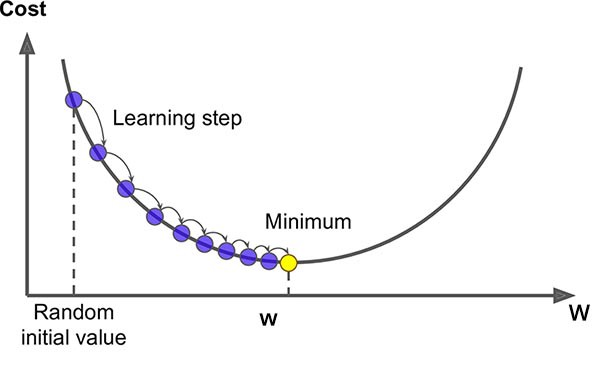
\includegraphics[width=0.9\columnwidth]{gradiente.jpg}
\caption{Visualización del Gradiente descendente, función de coste (Cost) y pesos (W).}
\label{fig:ejemplo}
\end{figure}

%-----------------------------------------------------------
\newpage
\subsection{Ejemplos}
En la figura de abajo vemos una ilustración del funcionamiento del algoritmo. En primer lugar, el punto inicial “0” es seleccionado aleatoriamente:

\begin{figure}[htbp]
\centering
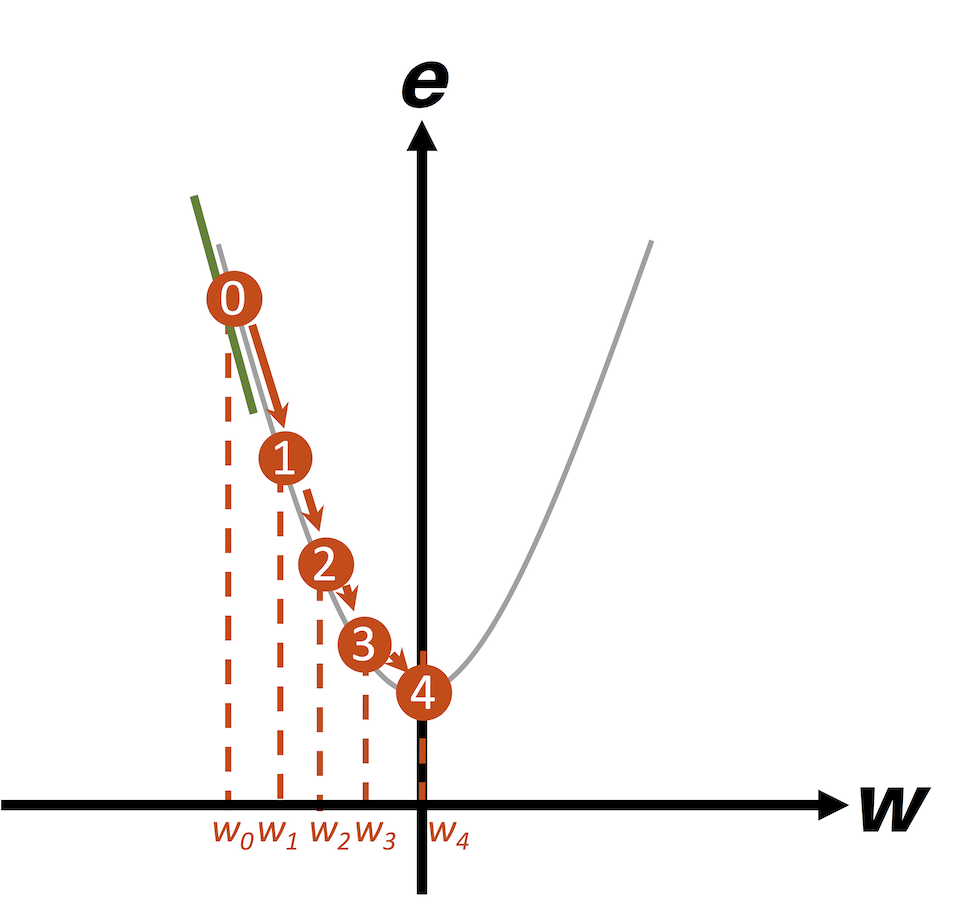
\includegraphics[width=0.4\textwidth]{ej1.png}
\caption{Descripción de la figura.}
\label{fig:ejemplo}
\end{figure}

En la primera iteración se calcula el gradiente en el punto $\omega_0$, que corresponde a la línea recta de color verde en la gráfica. Se observa que este gradiente es negativo, y por tanto la cantidad $-\alpha \cdot \text{gradiente}$ es un número positivo, lo cual quiere decir que al valor inicial de $\omega_0$ se sumará el término positivo $-\alpha \cdot \text{gradiente}$, y por tanto $\omega_1$ estará ubicado a la derecha del punto inicial.

En la segunda iteración el gradiente seguirá siendo negativo, y por tanto el término $-\alpha \cdot \text{gradiente}$ será nuevamente positivo, lo cual quiere decir que el nuevo valor $\omega_2$ estará ubicado a la derecha de $\omega_1$.

Si se repite el procedimiento podemos observar que en cada iteración el nuevo valor de $\omega$ calculado está cada vez más cerca del valor mínimo buscado ($\omega = 0$).

Algo similar ocurre cuando el punto inicial ($\omega$) es positivo, como se muestra en la figura de abajo:

\begin{figure}[htbp]
\centering
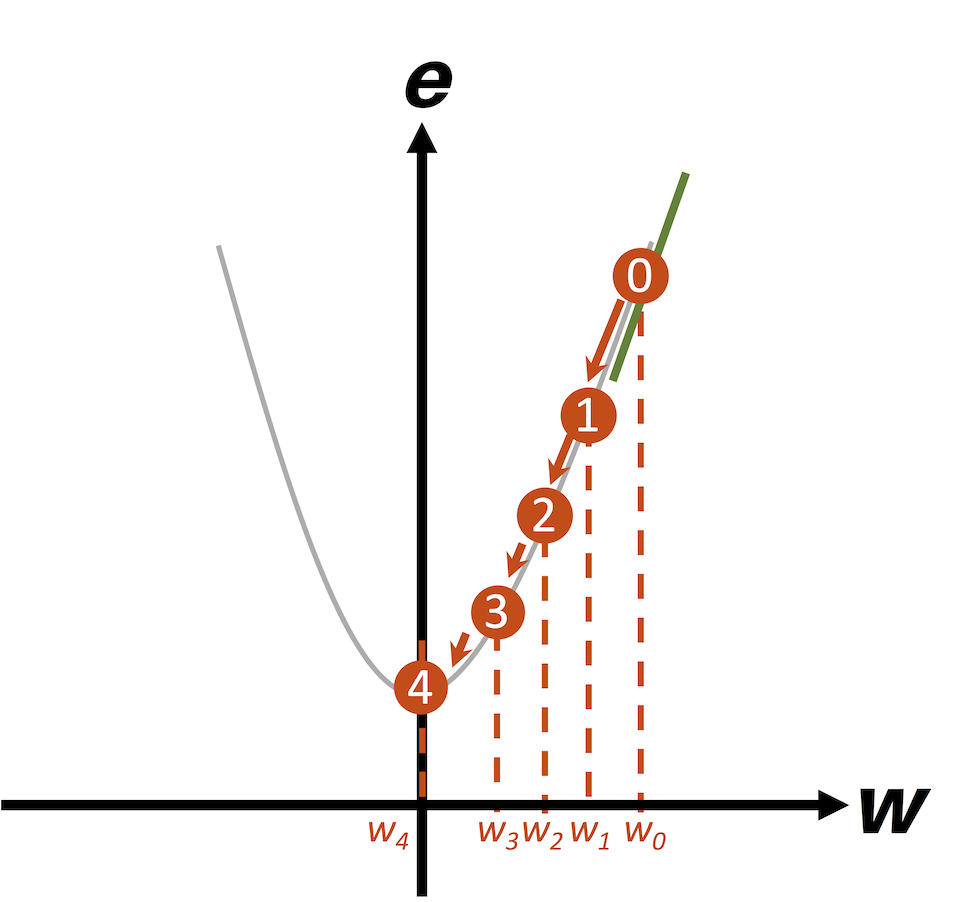
\includegraphics[width=0.4\textwidth]{ej2.png}
\caption{Ejemplo gráfico del gradiente descendente cuando el punto inicial (w) es positivo.}
\label{fig:ejemplo}
\end{figure}

El gradiente o derivada de la función \( e = \omega^2 + 1 \) es igual a \( 2\omega \). Para simular el comportamiento del algoritmo, supongamos inicialmente un valor \( \omega_0 = 5 \) y una tasa de aprendizaje \( \alpha = 0.25 \).

Así, en la primera iteración del algoritmo tendremos:

\begin{itemize}
    \item \( \omega_0 = 5 \)
    \item Gradiente \( \nabla e(\omega_0) = 2 \times 5 = 10 \)
    \item \( \omega_1 = \omega_0 - \alpha \cdot \nabla e(\omega_0) = 5 - 0.25 \times 10 = 2.5 \)
\end{itemize}

Al repetir el procedimiento obtenemos los siguientes resultados en las iteraciones 2 a 6:

\begin{itemize}
    \item \( \omega_2 = 1.25 \)
    \item \( \omega_3 = 0.625 \)
    \item \( \omega_4 = 0.3125 \)
    \item \( \omega_5 = 0.156 \)
    \item \( \omega_6 = 0.078 \)
\end{itemize}

Podemos observar que en este caso se requieren aproximadamente 6 iteraciones para que el valor de \( \omega \) sea casi cero.

Si ahora usamos una tasa de aprendizaje \( \alpha = 0.4 \), y repetimos el mismo procedimiento anterior, veremos que en lugar de 6 se requieren tan solo 3 iteraciones para que \( \omega \) alcance el valor de 0.04:

\begin{itemize}
    \item \( \omega_1 = 1.0 \)
    \item \( \omega_2 = 0.2 \)
    \item \( \omega_3 = 0.04 \)
\end{itemize}

Si consideramos la situación extrema \( \alpha = 1.0 \), observamos el siguiente comportamiento oscilatorio:

\begin{itemize}
    \item \( \omega_1 = -5 \)
    \item \( \omega_2 = 5 \)
    \item \( \omega_3 = -5 \)
    \item \( \omega_4 = 5 \)
    \item \( \omega_5 = -5 \)
    \item \( \omega_6 = 5 \)
\end{itemize}

Así, el valor de w alterna entre 5.0 y -5.0 y nunca disminuye. En este caso decimos que el algoritmo no converge y por tanto nunca encontrará un valor mínimo.\\

Los anteriores ejemplos nos permiten concluir que la tasa de aprendizaje $\alpha$ determina la cantidad de iteraciones requeridas para que el algoritmo del gradiente descendente alcance el valor mínimo, y el valor seleccionado dependerá de la función a minimizar (sin embargo siempre debe ser menor a 1).

%-----------------------------------------------------------
\section{Newton-Raphson}
Describa los métodos utilizados en su investigación. Incluya ecuaciones cuando sea necesario:
\subsection{Descripcion y/o deduccion del metodo}
Sea \( f:[a,b]\rightarrow\Re, f\in C^{2}[a,b]\) y \(x_k\) una estimación del cero en \( f:[a,b]\)

\textbf{Deducción del método}

Considere \( \Delta y_k = f'(x_k)*\Delta y_k\) con \( \Delta y_k\) apropiado \(  y_k = f(x_k)\) y además \( \Delta y_k = f(x_{k+1}) - f(x_k)\) 

Si \(  x_k\) es una aproximación de la solución  de \( f(x) = 0 \) en \( [a,b]\) y \(  x_{k+1}\) una mejor aproximación, \( f(x_{k+1}) \approx 0\) entonces:
\[
 \Delta y_k = -f(x_k) y  -f(x_k)=f'(x_k)* \Delta x_k
\]
así se obtiene:
\[
 \Delta x_k = -[f'(x_k)]^{-1}*f(x_k)
\]
con 
\[
\Delta x_k = x_{k+1} -x_k
\]

\subsection{Demostracion de orden convergencia}

Analicemos cuantitativamente el orden de convergencia. Dado un error pequeño $\delta_{n}$ en la $n$-ésima iteración, determinaremos cuánto más pequeño es el error $\delta_{n+1}$ en la siguiente iteración.

En particular, definimos $x_{n}=x(1+\delta_{n})$, donde $x=\sqrt{a}$ es la solución exacta. Esto corresponde a definir $|\delta_{n}|$ como el \textbf{error relativo}:

\[
|\delta_{n}|=\frac{|x_{n}-x|}{|x|},
\]

también llamado \textbf{error fraccional}. El error relativo es típicamente la forma más útil de cuantificar el error porque es una cantidad \textit{adimensional} (independiente de las unidades o escala de $x$). El logaritmo $(-\log_{10}\delta_{n})$ del error relativo representa aproximadamente el número de \textbf{dígitos significativos exactos} en la respuesta $x_{n}$.

Sustituyendo esta definición de $x_{n}$ (y $x_{n+1}$) en términos de $\delta_{n}$ (y $\delta_{n+1}$) en nuestra fórmula de iteración de Newton, y usando que $a/x = x$, podemos dividir ambos lados por $x$:

\[
1+\delta_{n+1}=\frac{1}{2}\left(1+\delta_{n}+\frac{1}{1+\delta_{n}}\right)=
\]

\[
\frac{1}{2}\left[1+\delta_{n}+1-\delta_{n}+\delta_{n}^{2}+O(\delta_{n}^{3})\right]
\]
donde hemos expandido $(1+\delta_{n})^{-1}$ en series de Taylor. La notación $O(\delta_{n}^{3})$ significa aproximadamente "términos de orden $\delta_{n}^{3}$ o superiores". Como la sucesión converge, podemos asumir que $|\delta_{n}|^{3} \ll 1$ para $n$ suficientemente grande, por lo que los términos $\delta_{n}^{3}$ y de orden superior son eventualmente despreciables frente a $\delta_{n}^{2}$. Obtenemos:

\[
\delta_{n+1}=\frac{\delta_{n}^{2}}{2}+O(\delta_{n}^{3}),
\]

lo que significa que el \textbf{error aproximadamente se cuadra} (y se reduce a la mitad) en cada iteración una vez cerca de la solución. Elevar al cuadrado el error relativo corresponde precisamente a duplicar el número de dígitos significativos, lo que explica el fenómeno observado. Esto se conoce como \textbf{convergencia cuadrática}, por lo tanto el método de Newton Raphson tiene convergencia cuadrática.
\subsection{Condiciones de estabilidad}
Según Burden (Sección 2.4, pp. 68--71), el método de Newton-Raphson es estable bajo las siguientes condiciones:

\subsection*{1. Condiciones Básicas de Convergencia}
\begin{enumerate}
    \item \textbf{Regularidad de $f$}:
    \begin{equation}
        f \in C^2([a,b]), \quad \text{donde } [a,b] \text{ contiene a la raíz } p.
    \end{equation}
    
    \item \textbf{No anulación de la derivada}:
    \begin{equation}
        f'(p) \neq 0.
    \end{equation}
    
    \item \textbf{Inicialización adecuada}:
    \begin{equation}
        |p_0 - p| < \delta, \quad \text{para } \delta \text{ suficientemente pequeño}.
    \end{equation}
\end{enumerate}

\subsection*{2. Teorema de Convergencia Cuadrática (Teorema 2.6)}
Si se cumplen las condiciones anteriores, entonces:
\begin{itemize}
    \item Existe una constante $M > 0$ tal que:
    \begin{equation}
        |p_{n+1} - p| \leq M |p_n - p|^2,
    \end{equation}
    lo que garantiza \textbf{convergencia cuadrática}.
    
    \item La cota del error depende de:
    \begin{equation}
        M = \frac{\max_{x \in [a,b]} |f''(x)|}{2\min_{x \in [a,b]} |f'(x)|}.
    \end{equation}
\end{itemize}

\subsection*{3. Casos de Inestabilidad}
\begin{itemize}
    \item \textbf{Raíces múltiples} ($f'(p) = 0$):
    \begin{equation}
        \text{Convergencia se reduce a lineal.}
    \end{equation}
    
    \item \textbf{Derivadas cercanas a cero}:
    \begin{equation}
        \text{Si } |f'(x)| \approx 0 \text{ cerca de } p, \text{ el método puede diverger.}
    \end{equation}
    
    \item \textbf{Elección inadecuada de $p_0$}:
    \begin{equation}
        \text{Si } p_0 \text{ está lejos de } p, \text{ no hay garantía de convergencia.}
    \end{equation}
\end{itemize}

\subsection{Comparacion de los metodos}

\section*{Diferencias entre el método de Newton y el Gradiente Descendiente}

\subsection*{Parametrización}
\begin{itemize}
    \item \textbf{Descenso de gradiente:} Es paramétrico según la tasa de aprendizaje $\alpha$.
    
    \item \textbf{Método de Newton:} No es paramétrico, lo que significa que podemos aplicarlo sin preocuparnos por la optimización de hiperparámetros.
    
    \item \textbf{Nota:} Existe una versión paramétrica del método de Newton, pero solo se aplica cuando operamos con una función polinómica con múltiples raíces.
\end{itemize}

\subsection*{Diferenciabilidad de la función}
\begin{itemize}
    \item \textbf{Método de Newton:} Presenta restricciones más estrictas en cuanto a la diferenciabilidad de la función.
    
    \item \textbf{Caso particular:} Si la segunda derivada $f''(x)$ no está definida en la raíz:
    \begin{itemize}
        \item Se puede aplicar descenso de gradiente
        \item No se puede aplicar el método de Newton
    \end{itemize}
\end{itemize}

\subsection*{Comportamiento en puntos estacionarios}
\begin{itemize}
    \item \textbf{Descenso de gradiente:}
    \begin{itemize}
        \item Si encuentra un punto estacionario durante la iteración, el programa continúa ejecutándose
        \item Los parámetros no se actualizan en este caso
    \end{itemize}
    
    \item \textbf{Método de Newton:}
    \begin{itemize}
        \item Requiere calcular $\frac{f'(x)}{f''(x)}$
        \item Para $f'(x) = f''(x) = 0$ se produce un error de división por cero
        \item El programa finalizaría con error en este caso
    \end{itemize}
\end{itemize}

\subsection{Ventajas y/o desventajas}

\section*{Ventajas del Método de Newton-Raphson}
El método de Newton-Raphson ofrece varias ventajas distintivas sobre otros métodos de búsqueda de raíces, especialmente en términos de velocidad, eficiencia y aplicabilidad a funciones suaves. A continuación, se presentan algunas ventajas clave:

\subsection*{A. Convergencia rápida (convergencia cuadrática)}
\begin{itemize}
    \item  El método de Newton-Raphson converge cuadráticamente cerca de la raíz, lo que significa que la cantidad de dígitos correctos aproximadamente se duplica con cada iteración, siempre que la estimación inicial esté cerca de la raíz verdadera.
\end{itemize}

\subsection*{B. Eficiente para funciones de buen comportamiento}
\begin{itemize}
    \item Cuando la función $f(x)$ es suave y su derivada $f'(x)$ es fácilmente calculable, el método de Newton-Raphson proporciona una búsqueda de raíces muy eficiente y rápida.
\end{itemize}

\subsection*{C. No es necesario el uso de corchetes}
\begin{itemize}
    \item A diferencia de métodos como la bisección y la falsa posición, el método de Newton-Raphson no requiere un intervalo de horquillado inicial. Solo se necesita una única aproximación inicial, lo cual puede resultar mucho más práctico.
\end{itemize}

\subsection*{D. Uso directo de información derivada}
\begin{itemize}
    \item El método de Newton-Raphson utiliza directamente la derivada $f'(x)$, lo que significa que puede incorporar más información sobre el comportamiento local de la función para converger más rápidamente.
\end{itemize}

\subsection*{E. Ampliamente aplicable a funciones suaves}
\begin{itemize}
    \item Cuando la función $f(x)$ es diferenciable, el método de Newton-Raphson es muy versátil y se puede aplicar a una amplia variedad de ecuaciones (incluidas ecuaciones trascendentales, algebraicas y trigonométricas).

 \end{itemize}

\section*{Desventajas del Método de Newton-Raphson}

\subsection*{A. Dependencia de la estimación inicial}
\begin{itemize}
    \item El método es muy sensible a la estimación inicial. Una mala elección de $x_0$ puede provocar:
    \begin{itemize}
        \item Divergencia del método
        \item Convergencia lenta
        \item Convergencia a una raíz local distinta a la deseada
    \end{itemize}
    \item Por lo tanto, el método puede requerir:
    \begin{itemize}
        \item Cuidadosa consideración de la estimación inicial
        \item Múltiples intentos con diferentes puntos de partida
    \end{itemize}
\end{itemize}

\subsection*{B. Cálculo de derivadas}
\begin{itemize}
    \item El método requiere el cálculo de la primera derivada $f'(x)$ de la función
    \item Problemas asociados:
    \begin{itemize}
        \item Para algunas funciones, el cálculo puede ser computacionalmente costoso
        \item En algunos casos la derivada puede ser difícil de obtener analíticamente
    \end{itemize}
    \item Alternativas:
    \begin{itemize}
        \item Métodos sin derivada (como el método de la secante) pueden ser más adecuados
        \item Uso de derivadas numéricas (aunque introduce error adicional)
    \end{itemize}
\end{itemize}

\subsection*{C. Falla en puntos críticos}
\begin{itemize}
    \item Casos problemáticos:
    \begin{itemize}
        \item Cuando $f'(x) = 0$ en la raíz o cerca de ella (división por cero)
        \item Cuando la función tiene singularidades cerca de la raíz
        \item Cuando existen puntos de inflexión cerca de la raíz
    \end{itemize}
    \item Consecuencias:
    \begin{itemize}
        \item El método puede fallar completamente
        \item Puede producir convergencia errática o no converger
    \end{itemize}
\end{itemize}

\subsection*{D. Raíces múltiples}
\begin{itemize}
    \item Problema fundamental:
    \begin{itemize}
        \item En funciones con múltiples raíces, el método puede converger a diferentes raíces dependiendo de la estimación inicial
    \end{itemize}
    \item Soluciones posibles:
    \begin{itemize}
        \item Técnicas de deflación para eliminar raíces encontradas
        \item Uso combinado con algoritmos de búsqueda global
        \item Aplicación del método desde múltiples puntos iniciales
    \end{itemize}
    \item Limitación adicional:
    \begin{itemize}
        \item Convergencia más lenta en raíces múltiples (orden de convergencia se reduce)
    \end{itemize}
\end{itemize}

\subsection{Elementos ilustrativos}
\begin{figure}[h]
    \centering
    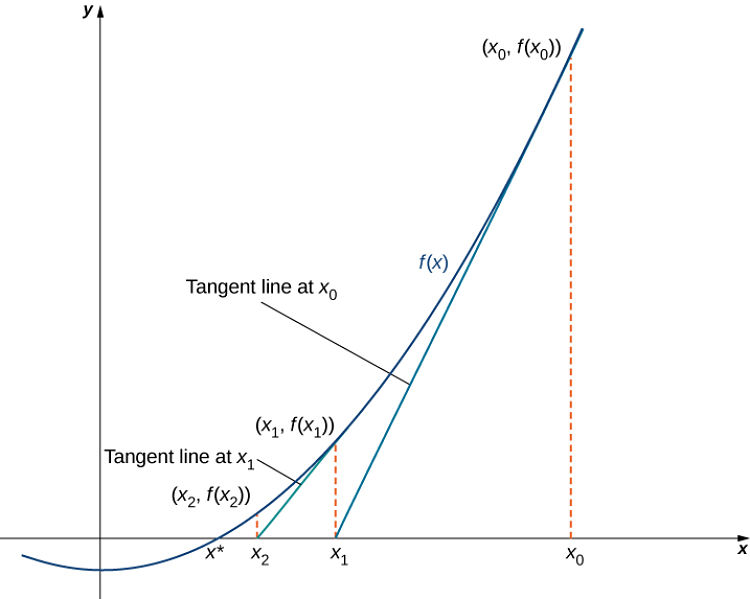
\includegraphics[width=0.9\linewidth]{newton.jpg}
    \caption{Visualización del método de newton}
    \label{fig:Newton}
\end{figure}
\subsection{Ejemplos}
\[f(x) = x^x e^{-x} \sqrt{2\pi x} - 120\]

\[\Rightarrow f'(x) = (f(x) + 120)\left[\ln x + \frac{1}{2x}\right]\]

\[\Rightarrow g(x) = x - \frac{f(x)}{(f(x) + 120)\left[\ln x + \frac{1}{2x}\right]}\]


El primer término de la función $f$ se denomina fórmula de Stirling, y es una aproximación a la función factorial. La solución de esta ecuación es aproximadamente 5 (cuyo factorial es precisamente 120).

En este ejemplo tomamos $x_0 = 6$ y $TOL = 10^{-6}$. En la tabla puede verse la evolución de la solución, y que converge en 6 iteraciones.

En este caso, el cero es simple y se observa la convergencia cuadrática esperada por la teoría.


\begin{center}
\begin{tabular}{c c c}
\toprule
$t$ & $x_i$ & $|x_i - x_{i-1}|$ \\
\midrule
0 & 6.0000000000 & -- \\
1 & 5.5568195217 & 0.0797543409 \\
2 & 5.2144604956 & 0.0656556949 \\
3 & 5.0438222496 & 0.0338311379 \\
4 & 5.0107677553 & 0.0065966925 \\
5 & 5.0097329283 & 0.0002065633 \\
6 & 5.0097319546 & 0.0000001944 \\
\bottomrule
\end{tabular}

[Fuente: Mantilla, Ignacio, ``Análisis Numérico'', Ejemplo 2.53]
\end{center}

% Conclusiones
\section{Conclusiones}
Los métodos de Gradiente Descendiente y Newton-Raphson son herramientas fundamentales en optimización numérica, cada una con sus ventajas y limitaciones. Mientras que el Gradiente Descendiente destaca por su simplicidad y eficiencia en problemas de alta dimensión, como los encontrados en aprendizaje automático, el método de Newton-Raphson ofrece una convergencia más rápida cerca del óptimo gracias al uso de información de segundo orden, aunque a un mayor costo computacional. La elección entre ambos depende del equilibrio entre precisión, velocidad y recursos disponibles, siendo clave considerar la naturaleza del problema, la dimensionalidad de los datos y la disponibilidad de derivadas. En muchos casos, técnicas híbridas o aproximaciones como los métodos quasi-Newton pueden ofrecer un balance óptimo entre rendimiento y eficiencia.

% Bibliografía-------------------------------------
\bibliography{referencias}
\begin{thebibliography}{1}

\bibitem{Machine_Learning}
“\textit{¿Qué es el machine learning?} - Explicación sobre el machine learning empresarial - AWS”. Amazon Web Services, Inc. Accedido el 16 de abril de 2025. [En línea]. Disponible: 
\href{https://aws.amazon.com/es/what-is/machine-learning/}{Link}

\bibitem{Gradiente_descendente} 
``¿Qué es el Gradiente Descendente?'' CodificandoBits.com. 
Accedido el 16 de abril de 2025. [En línea]. Disponible: 
\href{https://codificandobits.com/blog/el-gradiente-descendente/}{Link}

\bibitem{Gradiente_descendente2} 
IBM. “\textit{¿Qué es el descenso del gradiente?} | IBM”. IBM - United States. Accedido el 16 de abril de 2025. [En línea]. Disponible: \href{https://www.ibm.com/mx-es/think/topics/gradient-descent}{Link}

\bibitem{Gradiente_descendente2} 
J. A. SEPÚLVEDA ORTEGA, “\textit{IMPLEMENTACIÓN Y EXPERIMENTACIÓN CON MÉTODOS NUMÉRICOS DE OPTIMIZACIÓN DE PRIMER ORDEN EN SISTEMAS INERCIALES CON FACTOR DE AMORTIGUAMIENTO HESSIANO}”, TESIS PARA OPTAR AL GRADO MAGISTER EN CIENC. ING., MENCION MAT. APL., 2021. Accedido el 16 de abril de 2025. [En línea].\\ 
\href{https://repositorio.uchile.cl/bitstream/handle/2250/181490/Implementacion-y-experimentacion-con-metodos-numericos-de-optimizacion-de-primer-orden-en-sistemas-inerciales-con-factor-de-amortiguamiento-hessiano.pdf?sequence=1}{Link}
\bibitem{Newton_Raphson}
BRAVO BOLÍVAR, J. E., BOTERO ARANGO, A. J., and BOTERO ARBELÁEZ, M.  (2005). "\textit{EL METODO DE NEWTON-RAPHSON - LA ALTERNATIVA DEL INGENIERO PARA RESOLVER SISTEMAS DE ECUACIONES NO LINEALES}". Scientia Et Technica, XI(27), 221-224.[En linea]\\
\href{https://www.redalyc.org/pdf/849/84911698041.pdf}{Link}

\bibitem{gradienteVsNewton}
G. De Luca y M. Aibin. “gradient-descent-vs-newtons-gradient-descent”. www.baeldung.com. Accedido el 18 de abril de 2025. [En línea]. Disponible: 
\href{https://www.baeldung.com/cs/gradient-descent-vs-newtons-gradient-descent}{link}

\bibitem{Gradiente_estabilidad}
V. Patel, S. Zhang y B. Tian. “Global Convergence and Stability of Stochastic Gradient Descent”. List of Proceedings. Accedido el 18 de abril de 2025. [En línea]. Disponible: 
\href{https://proceedings.neurips.cc/paper_files/paper/2022/file/ea05e4fc0299c27648c9985266abad47-Paper-Conference.pdf}{link}

\bibitem{Gradiente_convergencia}
K. Ahn, J. Zhang y S. Sra. “Understanding the Unstable Convergence of Gradient Descent”. proceedings.mlr.press. Accedido el 18 de abril de 2025. [En línea]. Disponible: 
\href{https://proceedings.mlr.press/v162/ahn22a/ahn22a.pdf}{link}
\bibitem{Convergencia_newton}
Johnson, S. G. (s.f.). Newton's Method and the Sqrt Example [Notas de curso]. Departamento de Matemáticas, MIT.
\href{https://math.mit.edu/~stevenj/18.335/newton-sqrt.pdf}{Link}
\bibitem{Estabilidad-newton}
Burden, R. L., \& Faires, J. D. (2011). \textit{Numerical Analysis} (9th ed.). Cengage Learning.
\bibitem{Ventajas_desventajas_newton}
Ijraset. (s. f.). The Newton-Raphson Method: A Detailed analysis. IJRASET.
\href{https://www.ijraset.com/research-paper/newton-raphson-method-a-detailed-analysis}{Link}
\bibitem{Gradient_vs_newton}
De Luca, G.,  \& De Luca, G. (2024, March 18). Gradient Descent vs. Newton’s Gradient Descent Baeldung on Computer Science. Baeldung on Computer Science. 
\href{https://www.baeldung.com/cs/gradient-descent-vs-newtons-gradient-descent}{Link}
\end{thebibliography}



\end{document}